%
% 01_theorem.tex -- Einfuhrung in das Jordan'sche Kurventheorem
%
% (c) 2026 Dominik Castelberg, Ostschweizer Fachhochschule
%
% !TEX root = ../../buch.tex
% !TEX encoding = UTF-8
%
\section{Der Satz von Jordan \label{jordan:section:01_satz}}
\kopfrechts{Der Satz von Jordan}

Die meisten Theoreme der höheren Mathematik setzen ein tiefes Verständnis der zugrunde liegenden mathematischen Strukturen voraus, damit über ihre Korrektheit argumentiert werden kann. 
Andere Theoreme erscheinen jedoch derart trivial, dass ihre Korrektheit auf den ersten Blick offensichtlich ist und man zum Fehlschluss kommen könnte, dass ein Beweis überflüssig ist. 

\begin{theorem}[Satz von Jordan\label{jordan:theorem:jordan}]
    Sei $\gamma$ eine geschlossene, einfache Kurve in der Ebene $\mathbb{R}^2$. 
    Dann teilt $\gamma$ die Ebene in genau zwei zusammenhängende Gebiete: ein inneres Gebiet, das von $\gamma$ eingeschlossen wird, und ein äußeres Gebiet, das unendlich ausgedehnt ist. 
    Die Kurve $\gamma$ selbst bildet die gemeinsame Grenze dieser beiden Gebiete.
\end{theorem}

\begin{definition}[Geschlossene, einfache Kurve]
    Eine geschlossene, einfache Kurve $\gamma$ in der Ebene $\mathbb{R}^2$ ist eine stetige Abbildung $\gamma: [0,1] \to \mathbb{R}^2$, die folgende Eigenschaften erfüllt:
    \begin{enumerate}
        \item $\gamma(0) = \gamma(1)$ (die Kurve ist geschlossen),
        \item $\gamma(t_1) \neq \gamma(t_2)$ für alle $t_1, t_2 \in [0,1)$ mit $t_1 \neq t_2$ (die Kurve ist einfach).
    \end{enumerate}
\end{definition}

\begin{definition}[Grenze]
    Die Grenze eines Gebietes $G \subset \mathbb{R}^2$ ist die Menge aller Punkte $p \in \mathbb{R}^2$, für die jede Umgebung von $p$ sowohl Punkte aus $G$ als auch Punkte aus dem Komplement von $G$ enthält.
\end{definition}

\begin{definition}[Zusammenhängendes Gebiet]
    Ein Gebiet $G \subset \mathbb{R}^2$ ist zusammenhängend, wenn es nicht in zwei disjunkte, offene Teilmengen zerlegt werden kann. 
    Für jedes Paar von Punkten $p, q \in G$ existiert eine stetige Kurve innerhalb von $G$, die $p$ und $q$ verbindet.
\end{definition}

\begin{figure}
    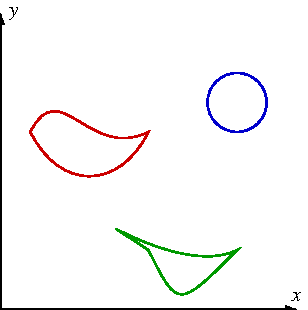
\includegraphics[width=0.8\textwidth]{papers/jordan/images/jordan_kurve.pdf}
    \caption{Beispiele für geschlossene, einfache Kurven}
\end{figure}

Das Satz von Jordan gehört zu den fundamentalen Resultaten der Topologie und hat weitreichende Anwendungen in verschiedenen Bereichen der Mathematik, der Physik und der Informatik. 
Seit seiner Formulierung im Jahr 1887 durch Camille Jordan versuchten Mathematiker, den Satz zu beweisen, wobei die ersten Versuche jeweils nach kurzer Zeit wieder verworfen wurden. 
Die Beweise waren oft unvollständig oder fehlerhaft, und es dauerte mehrere Jahrzehnte, bis der erste, allgemein als vollständig und rigoros anerkannte Beweis durch Oswald Veblen im Jahr 1905 veröffentlicht wurde.

Was macht diesen Satz so schwierig zu beweisen?

Die Schwierigkeit liegt primär in der generischen Formulierung des Satzes. Während es geradezu trivial ist, den Satz für spezielle Kurvenformen wie Kreise oder Ellipsen zu beweisen, wird die Komplexität des Beweises grösser, wenn man die Bedingung der Einfachheit und Geschlossenheit auf beliebige Kurven anwendet.

Stetigkeit wirkt nur als eine schwache Einschränkung auf die Kurve und erlaubt wilde Formen wie Fraktale, raumfüllende Kurven im Inneren oder Ränder mit positivem Lebesgue-Mass. All diese Beispiele sind über menschliche Intuition nur schwer zu erfassen und sind aufwändig zu analysieren, was die Beweisführung für den Satz von Jordan deutlich erschwert. 

\begin{definition}[Fraktal]
    Ein Fraktal ist eine geometrische Struktur, die auf allen Skalen selbstähnlich ist. 
    Fraktale können durch iterative Prozesse oder rekursive Algorithmen erzeugt werden und haben häufig nicht-integer Dimensionen.
\end{definition}

\begin{definition}[Lebesgue-Mass]
    Das Lebesgue-Mass ist eine mathematische Konstruktion, die es ermöglicht, die "Grösse von Mengen in einem Raum zu messen, insbesondere in $\mathbb{R}^n$. 
    Es verallgemeinert das Konzept der Länge, Fläche und Volumen auf komplexere Mengen, die nicht notwendigerweise reguläre geometrische Formen sind.
\end{definition}

